\chapter{Introduction}
\pagenumbering{arabic}
\setcounter{page}{1}

The speed of light in a vacuum is constant. This fact has enabled us to look
into the past and observe how the Universe has evolved over time. From the cosmic soup, to the emergence of the first stars, to the formation of galaxies; the evolution of the Universe has been a perennial source of fascination for mankind. One area of particular interest is the evolution of galaxies. Early on most galaxies were small, but gradually these smaller galaxies merged and amalgamated to form larger galaxies~\cite{mergingGalaxies}. Over time, as they continued to evolve, they began to manifest a great variety of galactic structures. However, this begins to raise a fundamental question: \textit{How does one classify the stages of evolution for a galaxy or determine where it is in its evolution}?

Hubble's Tuning Fork was the first classification scheme that sought to answer this, based on a galaxy's structure and size~\cite{hubblesTuningFork}. However, this scheme proved to be insufficient in the face of the complexity of the Universe and the variety of possible galactic formations~\cite{hubblesTuningFork}. An alternative approach to this classification scheme is to attempt to determine the age of galaxies based on their composition and not their overall shape. One such method involves determining the ages of various clusters of stars within a galaxy, thereby providing insight into the origin of the stars that constitute it.

Of the various cluster types, the globular cluster (\textit{GC}) is on average
the oldest~\cite{Jimenez1996}, and thus, the most significant in gauging the
age of galaxies. These types of clusters are stellar agglomerates~\cite{Gratton}
which formed in one of the following two ways~\cite{globular-cluster-formation}:
\begin{enumerate}
    \item Through the compression of halo gas in the cosmic re-ionization phase early on in the formation of the Universe.
    \item In the collapse of enormous molecular clouds triggered by events such as the collision of gas-rich galaxies.
\end{enumerate}
They are typically composed of around \num{10000} to \num{100000}
stars~\cite{sizeGC} bound tightly by gravity into a spherical formation. Some GCs are among the oldest objects in the Universe~\cite{OMalley2017} and are, thus, an interesting foundation for studying galactic evolution~\cite{Mohammadi}. These older GCs manifest some specific properties such as low metallicity~\cite{Dotter2011},
and through a combination of techniques, such as horizontal branch morphology, analysis of white dwarf cooling sequences, and comparisons using the main-sequence turn-off location~\cite{OMalley2017, Soderblom2010}, may have their age accurately determined, thereby setting the bounds for the age of the galaxy they are contained within. The question remains: \textit{How are these GCs found?}

\section{Existing Methods of Identifying GCs}

Astronomy is primarily an observational science, which, for most of its history, has gleaned information by looking up to the night sky with nothing but the naked eye. It was in this manner that the first GC, Messier 22,  was discovered. It was observed by Abraham Ilhe on August 6th, 1665 and as may be seen in Figure~\ref{fig:gc-m22} demonstrates an unusually dense core~\cite{Monaco2004}. This GC became the subject of much research across the 1900s and the statistics it has provided have been a basis for the identification of GCs today. The primary method for detecting new GCs has involved statistical analysis of photometric data across the Universe. Properties such as mean luminosity and metallicity are extracted from known GCs and are used to filter regions based on this spectroscopic information~\cite{gc-detection-old-1, Lee334}. To date, over 150 GCs have been discovered in our Milky Way, using such techniques~\cite{Harris2010}.

\begin{figure}[H]
    \centering
    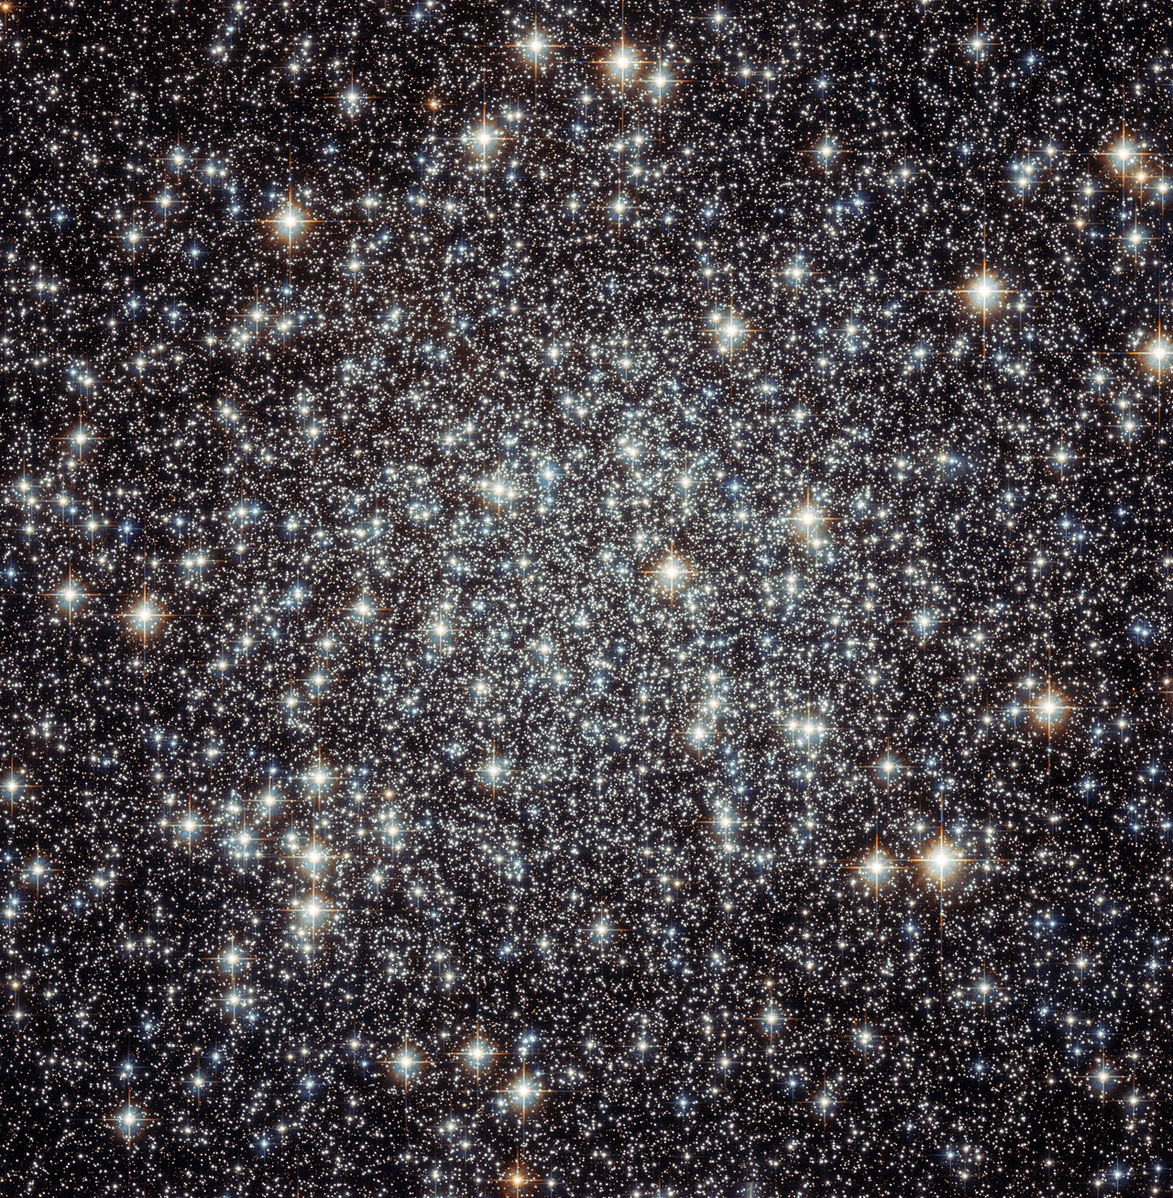
\includegraphics[width=0.45\textwidth]{img/m22.jpg}
    \caption{\label{fig:gc-m22} Crammed Center of Messier 22 taken by ESA/Hubble~\cite{wikimedia-gc-m22}}
\end{figure}

As a brief interlude, the advent of the large-scale tools used in modern astronomy have allowed for the collection of enormous amounts of information within our galaxy and far beyond. Telescopes (refractory, reflector, radiography, spectrography, and x-ray) allow us to extract a variety of information all without leaving the Earth's surface~\cite{Yuan-SenTing2014}. To collect information without the interference of the Earth's atmosphere we make use of satellites and space observatories that have been launched into orbit around our planet~\cite{8thGradeScience}. Occasionally, a space probe will be sent beyond our orbit to collect information from asteroids, planets, or their moons within our solar system~\cite{8thGradeScience}. However, for stellar observations, the use of telescopes becomes necessary due to the sheer distances involved. Thus, the techniques used for the identification of GCs were predominantly limited to the evaluation of photometric data and performing statistical analysis.

However, this has changed with the first Gaia data release in September 2016. In this data-set stars are represented by IDs and are coupled with a variety of astrometric, photometric, and spectroscopic readings~\cite{gaiaMission} (see Chapter~\ref{chap:data} for details). This allows processing to occur on a per-star basis and allows for a greater variety of techniques to be employed. The state-of-the-art in GC detection across such data-sets is described by Mohammadi et al.\ in 2018~\cite{Mohammadi}. In their paper, they make use of 3D kernel density estimations (\textit{KDE}) across subdivisions of the data-set. Using these estimations they then evaluated two different techniques:
\begin{itemize}
    \item Nearest-neighbors search.
    \item Kernel based anomaly detection through the training of a support-vector machine on random portions of the sky to search for outliers.
\end{itemize}
For both techniques, they then use a blob-detection technique based on Difference of Gaussian, as a post-processing method to further filter the regions.

\section{Objectives}

The research in this paper follows from the work of Mohammadi et al.\ and seeks to automate the discovery of potential GCs using data from stellar catalogs such as the Gaia data-set. The objective is to produce a pipeline using:
\begin{enumerate}
    \item \hyperref[sec:DoG]{Blob-detection}: based on Difference of Gaussian (\textit{\blobdog{}}), as a crude initial filter that reduces the number of candidate regions for further inspection.
    \item \hyperref[sec:Ant]{Ant Colony random-walk algorithm}: to compute density information in the form of pheromone values.
    \item \hyperref[sec:Clustering]{Clustering}: via an algorithm which pools these pheromone values in 3D space gravitationally to determine clusters.
\end{enumerate}

This pipeline is optimized and tested on data from the Gaia DR2 data-set~\cites{gaiaMission, gaiaDr2}. Different regions consisting of a variety of stellar objects are selected. Some of these regions contain previously found GCs, while some do not. Since we cannot state with absolute certainty the total number of GCs (for any given region, more may yet be found), the accuracy of the pipeline is explored by running it on these different regions and then evaluating it in two ways. First, we determine if it finds all \hyperref[tb:known-gcs]{known GCs}, and second we consider what other stellar structures (if any) it classifies as GCs.

A robust classifier for GCs would be a useful addition to the tool-set for exploring the Universe and its utility could be further evaluated with the full publication of the Gaia DR3 data-set slated for release in the first-half of 2022~\cite{GaiaDR3}.

It is important to note that due to the scope of this project, the emphasis does not lie in precisely optimizing the parameters associated with the pipeline.
The aim is to identify the effectiveness and shortcomings of the individual stages of the pipeline, as well as to identify potential parametric relationships between the different stages.

\section{Summary}

The rest of this paper is structured as follows:

First, we take a closer look at the Gaia Data Release 2 in
Chapter~\ref{chap:data}. We begin by depicting the stellar regions under
evaluation. This is followed by a description of various astronomical objects
that will be of interest in the analysis. Additionally, the parameters that will
be made use of from the data-set are scrutinized.

In the chapter on methodology, Chapter~\ref{chap:methodology}, the overview of
the pipeline is provided. This is coupled with in-depth descriptions of the
three techniques in use, namely, Difference of Gaussian, the Ant
Colony algorithm, and the Gravitational Clustering algorithm.

The results are explored in Chapter~\ref{chap:results}, which discusses the
findings for the individual components of the pipeline. Additionally, it includes the
statistical results and plots which reveal interesting characteristics of the
pipeline. The results for the regions are compared and contrasted to
explore the differences.

In Chapter~\ref{chap:conclusion}, conclusions are drawn about the effectiveness of the pipeline based on the results and discusses how they compare against the objectives that were set forth.

In Chapter~\ref{chap:evaluation}, the results are interpreted and evaluated to provide an insight into how well the individual components of the pipeline have worked, and attempts to learn from the successes and shortcomings. It also describes worthwhile avenues for further research.
